\label{third part}
\subsection{Introduction}

This part focuses on how the \emph{Monte Carlo Tree Search} is parallelized as a means of optimization. A classic \emph{MCTS} is an algorithm which sequentially creates random developments of the game. In order to speed up the results, develop more nodes of the tree search or even have more realistic statistics,the exploration of the tree will be parallelized. It means that parts of the tree development will be distributed to multiple threads, among multiple computers. Therefore, each thread on each computer will have less executions and the algorithm will be more efficient.
\newline
\newline

Currently, there are three principal strategies about how to parallelize the tree. They are called: Leaf Parallelization, Root Parallelization and Tree Parallelization\cite{parallel_comp, master_mcts_kozeleck}.

\subsection{Leaf Parallelization}
\label{sec:leaf}

The Leaf Parallelization is the easiest way to parallelize the exploration of the tree. In this method, only one thread traverses the tree and adds one or more nodes to the tree when the leaf node is reached. Then a set of threads is created, each one playing the game independently Once they all have finished, they back-propagate their results to the leaf and then, a single thread changes the tree’s global results. The Leaf Parallelization method is depicted in figure \ref{comp_algo}.
\newline
\newline

The advantage of this method is that its implementation seems very simple. The threads do not need to be synchronized. However, there are two significant problems.
\begin{itemize}
     \item The time consumed by a thread to finish the game is unknown. Therefore, it will take, on an average, more time to do n games with n threads, than one game with one thread, since this method waits for the last one.
     \item There is no communication between the threads. If a majority of the threads (the faster ones) have led to a loss, it would be very likely that all of them lead to a loss. And so, the last thread will be executed for nothing. 
  \end{itemize}

\subsection{Root Parallelization}
\label{sec:root}

The second method is the Root Parallelization. It consists in giving each thread the same tree during the same amount of time. They will independently and randomly develop their tree and, at last, they will merge all of the results. This method can also be called \emph{Single-run parallelization} or \emph{Slow-Tree Parallelization}, and is depicted in figure \ref{comp_algo}.
\newline

Its biggest advantage is also one of its drawbacks. Indeed, the threads do not communicate with each other. On one hand, it means there is some redundancy in the development of the tree. On the other hand, the lack of communication drastically increases the speed of the program. Actually, the strength of this strategy lies in little communication.

\subsection{Tree Parallelization}
\label{sec:tree}

Finally, the third method is called the Tree Parallelization. In this method, multiple threads share the same tree and can randomly choose a leaf to develop it. The main problem of this method is that multiple threads can access the same node and corrupt data given by another thread. To prevent this corruption there is two main methods proposed by Guillaume Chaslot, Mark Winands, and H. Jaap van den Herik \cite{parallel_comp}. The first one is to use mutexes, or mutual exclusions (mutex), on the tree and the second is to implement a virtual loss. The first method is depicted in figure \ref{comp_algo}. The other one is explained below.
\newline

The mutexes can be either global or local. The global mutexes block access to the whole tree when a thread is accessing it. The time loss induced by the mutexes increases with the number of thread, up to a point where ading another thread does not cause any time gain. The local mutexes block only the node that the thread is using in order not to block the entire tree. This method is better but still implies an important number of locking and unlocking. However, fast-access mutexes and spinlocks can be used to increase the speed of the program.
\newline

Nevertheless, according to Markus Enzenberger and Martin Müller \cite{lock-free}, by the lack of mutexes, the problem of the data corruption is negligible compared to the speed decrease of the program, especially when the number of threads exceeds two. Therefore, one can assume that, to be the most efficient, one can simply eliminate mutexes.
\newline

The second method, the virtual loss, consists in decreasing the value of the node that the first thread accesses. When the second thread searches a node to develop, it will only take this node if it is considerably better than the others. This strategy allows nodes with high probability of winning to be visited by multiple nodes and avoid redundancy on the other ones.

\subsection{Hybrid Algorithms}

Research about hybrids technologies of parallelization has been investigated. Those technologies use a mix of the parallelization methods eplained in sections \ref{sec:leaf}, \ref{sec:root} and \ref{sec:tree}. Some parallelization strategies are a combination of multiple methods with some additional content, but they are very complex to compute and are efficient in specific cases.


\subsubsection{UCT-Treesplit}

The \emph{UCT-Treesplit} algorithm\cite{treesplit} retakes the base of \emph{Root Algorithm} and makes it work on clusters which can compute the nodes. %not sure that was what you meant
It is depicted in figure \ref{treesplit}. It’s made for High-Performance Computers (or \emph{HPC}) which have cluster parallelization and shared memory parallelization. Moreover, this method demands a lot of communication and so, the network latency is a very important factor of slow-down.

\begin{figure}[!h] 
\centerline{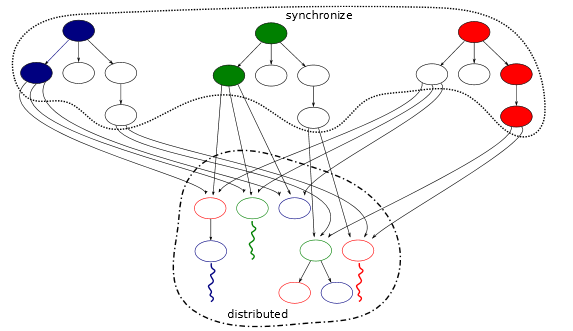
\includegraphics[scale=0.60]{2_State_of_the_art/Strategy_of_root_parallelization_Mikail/treesplit.png}}
   \caption{\label{étiquette} UCT-Treesplit overview}
\label{treesplit}
\end{figure}

\subsubsection{Block Parallelization}

Another efficient hybrid algorithm is the \emph{Block Algorithm}\cite{GPU}.  It is depicted in figure \ref{block}. It is working by giving some instructions to GPU\footnote{GPU: Graphics Processing Unit, processor dedicated to graphics} and some other instructions to CPU\footnote{CPU: Central Processing Unit, main processor on the computer}. The Block Parallelization is a blending of \emph{Leaf Algorithm} and \emph{Root Algorithm}. As GPUs can run hundreds of threads, it is used to develop a specific node with the \emph{Leaf Algorithm} whereas CPU is used to develop the trees using the \emph{Root Algorithm}.The benefit of this method is that each of these components are used in the way they were meant to be used.

\begin{figure}[!h] 
\centerline{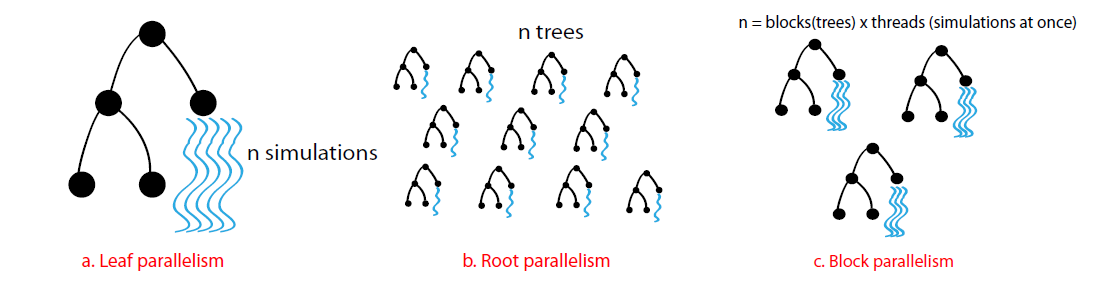
\includegraphics[scale=0.60]{2_State_of_the_art/Strategy_of_root_parallelization_Mikail/block.png}}
   \caption{\label{étiquette} Scheme of the Block Parallelization comparing to Leaf and Root}
\label{block}
\end{figure}

\subsection{Comparison of simple strategies}
\begin{figure}[!h] 
\centerline{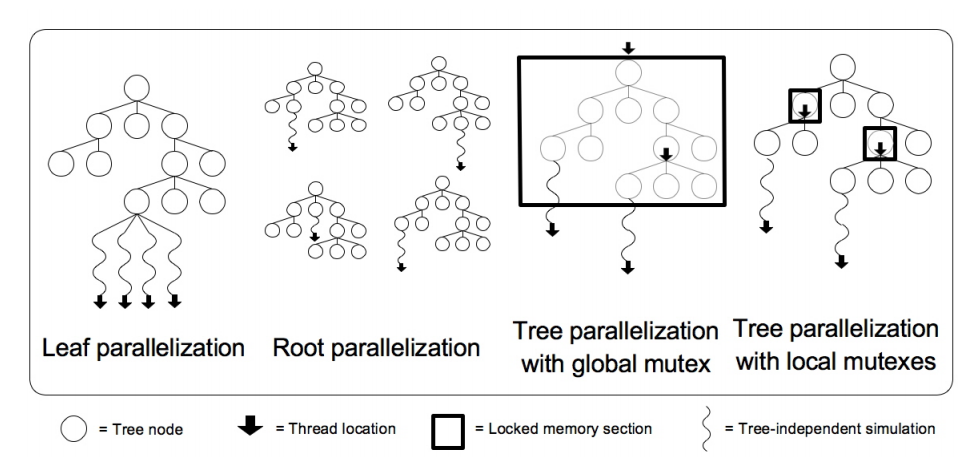
\includegraphics[scale=0.60]{2_State_of_the_art/Strategy_of_root_parallelization_Mikail/impara.png}}
   \caption{\label{étiquette} Comparison of all trees}
\label{comp_algo}
\end{figure}

Currently, the best strategy to adopt is the \emph{Root Parallelization} on those specific test conditions. According to some tests \cite{parallel_comp,tree_root_comp}, the advantages of the \emph{Root Parallelization} is its drawbacks. Indeed, for 16 threads, a program using \emph{Root Parallelization} will win 56\% of the time against 36.5\% for the \emph{Leaf Parallelization}, and 49\% for the \emph{Tree Parallelization} with the use of a virtual loss. Moreover, the \emph{Root Parallelization} is always twice as fast as the \emph{Tree Parallelization} with virtual loss. It can be explained by the fact that numerous trees are massive and so much time will be lost doing communication and synchronization. None of these issues exist with the \emph{Root Parallelization}. Furthermore, this method is also very simple to implement.

\subsection{Conclusion}

The strategy used to parralelize the algorithm depends on the hardware that will be used. Since both cluster parallelization and shared memory parallelization will be used, a simple \emph{Root Parallelization} between the different computers can be chosen, in addition to an algorithm specialized in shared memory parallelization, like \emph{Tree Parallelization}. If the use GPU is preferred over the CPU or even both of them, \emph{Block Parallelization} is used. Also, if the network and the computers are fast, UCT-Treesplit can be used to parallelize the algorithm.
